%!TEX root = ../my_thesis.tex

\graphicspath{{main/chapter1/fig/}}

\chapter{Context and Objectives}
\label{chap:ctx}

\vspace*{\fill}
\minitoccustom
\vspace*{\fill}

\section{Digital Communication Systems}

% \begin{itemize}
%   \item Shannon~\cite{Shannon1948}: système de communication (source -> émetteur
%     -> canal -> récepteur -> destination)
%   \item utilisé partout dans notre monde (télé, téléphone, internet, satellites,
%     etc.)
%   \item zoom sur l'émetteur (source -> codage canal -> modulation)
%   \item zoom sur le récepteur (démodulation -> décodage canal -> destination)
%   \item introduction au codage canal, nécessaire pour mieux résister aux
%     perturbations dues à la traversée du signal dans un environnement physique
%     (le canal)
%   \item modulation: représentation d'une information numérique en analogique
%     adaptée au canal
%   \item évoquer la synchro avant la démodulation
%   \item couche physique (PHY 1) du modèle OSI
%   \item couche physique traditionnellement implémentée en hardware (ASIC)
%   \item récepteur gourmand en calcul (plus particulière l'algorithme de décodage
%     et un peu la démodulation)
% \end{itemize}

\begin{figure}[htp]
  \centering
  \includegraphics{intro/com_chain/com_chain}
  \caption{Digital communication chain.}
  \label{fig:intro_com_chain}
\end{figure}

It is now commonplace to state that Humanity has entered the era of
communication. By 2025, there should be more than 5 billion smart-phones in
circulation worldwide. Moreover, all kinds of objects will increasingly also use
communication technology, to exchange information in the \emph{Internet of
Things} (IoT) for instance. Despite their variety, all communication systems are
based on a common abstract model proposed by Claude Shannon. In his seminal
paper~\cite{Shannon1948}, he proposed to model a communication system with five
components: an information source, a transmitter, a channel, a receiver and a
destination. This model was later refined as shown in
Figure~\ref{fig:intro_com_chain}. The source produces a digital message $\bm{u}$
to be transmitted (sequence of bits). The channel encoder transforms it in a
codeword $\bm{c}$ to make it less prone to errors. In order to make possible the
information transmission through the channel, it is necessary to shape the data
stream. For instance, in the case of wireless communication, this stream must be
represented by a high-frequency signal in order to be transmitted by a
reasonably sized antenna. This is the role of the digital modulator which
produces a vector of symbols $\bm{x}$. The channel alters the signal with some
noise and distortions ($\bm{y}$). On the receiver side, the components perform
the inverse operations to retrieve the message $\bm{\hat{u}}$ produced by the
source.

In channel coding, also known as \emph{forward error correction}, $K$
information bits  are encoded in the transmitter. It results in a codeword
$\bm{c}$ of $N$ bits. $P = N - K$ is the number of parity bits added as
redundant information and $R = K/N$ is the code rate. Higher the code rate $R$
is, lower the number of parity bits $P$ is. The performance of this chain is
measured by estimating the residual error rate at the sink. More precisely, it
is possible to observe two different rates: 1) the Bit Error Rate (BER); 2) the
Frame Error Rate (FER). The BER is calculated considering the $K$ information
bits independently, for instance a $10^{-3}$ BER means that there is an average
of one binary error per thousand bits transmitted. The FER is computed
considering the entire frame, if there is one, two or more wrong bits in the
current frame, it will be counted as one error frame. A $10^{-2}$ FER means that
there is an average of one frame error per hundred frame transmitted. These
rates are directly driven by the choice of the channel encoder and decoder.
Lower the rates are, higher the correction power of the system is.

\section{Channel Model}

In this thesis, only causal transmission channels without memory effect and
stationary are considered. In other words, the output of the channel at time $t$
only depends on its input at time $t$. In order to describe the disturbance to
the message $\bm{x}$ passing through the transmission channel, different
models can be used. However, in the literature, the selected model is very
often the Additive White Gaussian Noise (AWGN) channel. In particular, this
channel models very well the thermal noise which is one of the sources of
noise always present on the receiver side.

In the AWGN channel, the law binding the $y_i$ output to its $x_i$ input is of
the form $y_i = x_i + n_i$ with $N_{chn}$ an independent and identically
distributed variable according to a normal (or Gaussian) law centered in zero
and of variance $\sigma^2 = N_0 / 2$. So, we have $N_{chn} \simeq \mathcal{N}(0,
\sigma^2)$ and:
\begin{equation}
P_r(y_i|x_i) = \frac{1}{\sqrt{2\pi\sigma^2}}\exp{\Big(-\frac{(y_i-x_i)^2}{2\sigma^2}\Big)}.
\end{equation}

To estimate the correction power of a system it is very common to vary the
Signal-to-Noise Ratio (SNR). On the AWGN channel the SNR is generally given by
$E_b/N_0$ (in dB). $E_b$ corresponds to the average energy per information bit.
It can also be given by $E_s/N_0$ (in dB) where $E_s$ corresponds to the average
energy per transmitted symbol. $E_s/N_0$ can be deduced from $E_b/N_0$:
\begin{equation}
\frac{E_s}{N_0} = \frac{E_b}{N_0} + 10.\log{(R.b_S)},
\end{equation}
where $R$ is the code rate and $b_S$ is the number of bits per transmitted
symbol $x_n$. $b_S$ depends on the modulation order, if a simple binary modulation
is used, then $b_S = 1$. Then, the Gaussian variance $\sigma$ of AWGN channel
comes:
\begin{equation}
\sigma = \sqrt{\frac{1}{2 \times 10^{\frac{E_s}{N_0} / 10}}}.
\end{equation}

An important characteristic of a channel is its capacity~\cite{Ryan2009}. The
capacity represents the maximal quantity of information that the canal can
transport. In other terms, it is impossible to find a coding scheme that
transports more information than the channel capacity.
From this capacity it is possible to deduce the Shannon's
limit~\cite{Shannon1948}. This limit is the asymptotic SNR in $E_b/N_0$ (dB)
which cannot be beaten with any channel code. When $R$ tends towards zero it can
be shown that the Shannon's limit is $-1.59$ dB. This means that, for an AWGN
channel, no system can reliably transmit information at a SNR of less than
$-1.59$ dB.

In the next chapters of the manuscript, the AWGN channel will mainly be
associated with a Binary Phase-Shift Keying (BPSK) modulation ($b_S = 1$). With
this modulation, each binary value $c_i \in \{0,1\}$ is associated to a real
value $x_i \in \{-1,1\}.$ The $\bm{l}$ outputs estimated by the digital
demodulator are given in the form of a Log Likelihood Ratio (LLR). Their sign
determines for each channel output data $y_i \in \bm{y}$ the most probable
binary input $c_i \in \bm{c}$. The absolute value corresponds to the degree of
reliability of the information. The mathematical expression for $l_i$ is:
\begin{equation*}
l_i = \log{\Big(\frac{P_r(y_i|c_i = 0)}{P_r(y_i|c_i = 1)}\Big)}.
\end{equation*}

\section{Capacity-approaching Channel Codes}

After Shannon, researchers have designed new coding/decoding schemes to approach
Shannon's theoretical limit even closer. Indeed, recent progresses managed to
design practical codings performing very close to that limit, and are already
integrated in everyday communication systems. These code are habitually
classified in two distinct families: block codes and convolutional codes. By
definition the convolutional codes compute the redundancy in continue on the
data stream while the block codes generate the redundancy by chunks of data.
The purpose of this section is to detail a little bit the construction of the
most famous ones, namely LDPC, turbo and polar codes.

\begin{table}[htp]
  \centering
  \caption{Elementary operations in $GF_2$ (logical \emph{exclusive or} and
    {and}).}
  \label{tab:ctx_gf2_operations}
   \begin{tabular}{c c c c}
   $a$ & $b$ & $a \oplus b$ & $ab$ \\
    \hline
    \hline
    0 & 0 & 0 & 0 \\
    0 & 1 & 1 & 0 \\
    1 & 0 & 1 & 0 \\
    1 & 1 & 0 & 1 \\
  \end{tabular}
\end{table}

In all the presented coding schemes, only binary codes are considered. In this
case, a bit can be represented by a Galois field of two elements $\{0, 1\}$
denoted as $GF_2$. A block code is an application $g$ of $GF_2^K$ in $GF_2^N$
with $K < N$. There is $2^K$ codewords $\bm{c}$. The two operators used to
generate a codeword are the addition and the multiplication. In $GF_2$, the
addition is equivalent to the \emph{logical exclusive or} (XOR or $\oplus$) and
the multiplication is equivalent to the \emph{logical and} (cf.
Table~\ref{tab:ctx_gf2_operations}).

\subsection{LDPC Codes}

The Low-Density Parity-Check (LDPC) codes are linear block codes, they have been
discovered very early by Robert G. Gallager in 1962~\cite{Gallager1962}.
Unfortunately, at the time of their discovery, the computational power available
in the transceivers was not sufficient to use them. But, in 1995, the LDPC codes
have been re-discover by David MacKay~\cite{MacKay1995} and used in many digital
communication standards since (Wi-Fi, WiMAX, WRAN, 10Gbps Ethernet, DVB-S2,
CCSDS, 5G, etc.).

% LDPC codes is a family of channel codes that is well spread in current digital
% communication systems. They have been chosen in many communication standards
% (Wifi, WiMAX, DVB-S2, 10Gbps Ethernet, etc.). They were also selected for the
% future 5G standard data transport.

\subsection{Turbo Codes}

The turbo codes have been discovered by Claude Berrou in 1993~\cite{Berrou1993}
and have been used in many digital communication standards since (3G, 4G,
DVB-RCS2, CCSDS, etc.). Unlike the LDPC codes, the turbo codes are convolutional
codes. The particularity of the turbo codes is to be composed by two sub-codes.
In other terms, the turbo codes are a parallel concatenation of two
convolutional codes.

\subsection{Polar Codes}

The polar codes are linear block codes like the LDPC, they have been discovered
relatively recently by \Arikan in 2009~\cite{Arikan2009} and are used in the
5G standard. The particularity of these codes is that they are the only ones for
which it has been mathematically demonstrated that they reach the Shannon's
limit (considering an infinite codeword length).

\subsection{Other Codes}

\begin{itemize}
  \item \xmark~parler rapidement des codes BCH, RS, TPC...
  \item \xmark~codes non binaires et polar multi-kernel ?
  \item \xmark~dire que la liste n'est pas exhausive et qu'il y a pleins
    d'autres codes dont on ne parle pas ici
\end{itemize}

\section{Simulation}

There are many possible coding schemes with different characteristics. The
previous section presented different codes used in most of the today standards.
Before they were standardized, these codes have been compared an evaluated.
The codes can be constructed in a infinity of different way and for each coding
scheme, many different decoding algorithms can be implemented. It is then
mandatory to be able to evaluate and compare the BER/FER decoding performance of
the selected codes with each others before to implement them in real systems. To
this purpose, the channel coding specialists massively use the simulation.
Depending on the channel model it is possible to predict with varying degrees of
ease (in term of computational effort) the BER/FER decoding performance of a
communication system. For simple channel models it is possible to evaluate
analytically the performance but when the channel model complexity increases it
becomes impossible to use direct methods. This is especially the case with the
AWGN channel presented before. The solution is then to resort to a compute
intensive Monte Carlo simulation of the communication system. The idea is to
evaluate the performance of the system by generating many random frames and
applying random noise samples on these frames, then the noisy frames are decoded
and the output sequence of bit $\bm{\hat{u}}$ is compared with the initial
information bits $\bm{u}$.

\begin{figure}[htp]
  \centering
  \subfloat[][Specification of the processing chain.]
  {
    \includegraphics[scale=1]{simu/com_chain/com_chain}
    \label{fig:simu_com_chain_specs}
  }
  \\
  \subfloat[][Input simulation parameters and output BER results.]
  {
    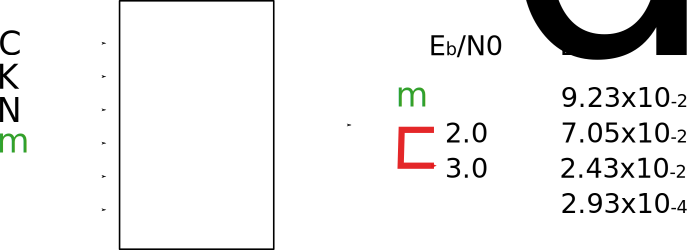
\includegraphics[scale=1]{simu/in_out/in_out}
    \label{fig:simu_com_chain_in_out}
  }
  \caption{Example of a digital communication system simulation.}
  \label{fig:simu_com_chain}
\end{figure}

Fig.~\ref{fig:simu_com_chain_specs} describes a processing sequence similar
to the digital communication chain presented in Fig.~\ref{fig:intro_com_chain}.
The only difference is that the \emph{sink} block has been replaced by what we
call a \emph{monitor}. The \emph{monitor}, unlike the \emph{sink}, knows the $K$
output information bits from the \emph{source} ($\bm{u}$). The $C$, $K$ and $N$
parameters are, respectively, the type of the code, the number of information
bits and the codeword size. These parameters have a direct impact on the
selection of the \emph{channel encoder} and the \emph{channel decoder} blocks
in the simulation. Fig.~\ref{fig:simu_com_chain_in_out} shows the BER output of
the simulation. The $m$, $M$ and $s$ parameters allow to control the AWGN
channel noise. $m$ is the minimum SNR value to simulate in the channel, while
$M$ is the maximum SNR value. $s$ is the SNR step between two SNR values.

Fig.~\ref{fig:intro_bfer} presents BER and FER decoding performances estimated
with Monte Carlo simulations on a large variety of code families and decoding
parameters. On each graphic, the BER is plotted with solid lines while the FER
is plotted with dashed lines. Both the BER and the FER depend on the SNR
($E_b/N_0$). Higher the SNR is, less there is noise and therefore fewer errors.
For instance, in Fig.~\ref{fig:intro_bfer_polar}, considering a noise of 4.5 dB,
the FA-SCL with $L = 32$ decodes better than the FA-SCL with $L = 8$ because
the {\color{Paired-1} blue} curve is below the {\color{Paired-5} red} curve. In
other terms, lower is better. The purpose of Fig.~\ref{fig:intro_bfer} is not
to compare the codes with each others but to introduce the typical BER/FER plots
that will be used in the next chapters and to show that there is a large set of
possible combinations of codes and parameters.

\begin{figure}[htp]
  \centering
  \subfloat[][Polar codes.]        {\includegraphics[width=0.30\textwidth]{simu/bfer/bfer_polar} \label{fig:intro_bfer_polar}}  \quad{}
  \subfloat[][LDPC codes.]         {\includegraphics[width=0.30\textwidth]{simu/bfer/bfer_ldpc}  \label{fig:intro_bfer_ldpc}}   \quad{}
  \subfloat[][Turbo codes.]        {\includegraphics[width=0.30\textwidth]{simu/bfer/bfer_turbo} \label{fig:intro_bfer_turbo}}  \\
  \subfloat[][Turbo product codes.]{\includegraphics[width=0.30\textwidth]{simu/bfer/bfer_tpc}   \label{fig:intro_bfer_tpc}}    \quad{}
  \subfloat[][BCH \& RS codes.]    {\includegraphics[width=0.30\textwidth]{simu/bfer/bfer_bch_rs}\label{fig:intro_bfer_bch_rs}} \quad{}
  \subfloat[][Convolutional codes.]{\includegraphics[width=0.30\textwidth]{simu/bfer/bfer_rsc}   \label{fig:intro_bfer_rsc}}
  \caption{Simulation outputs of various code families.}
  \label{fig:intro_bfer}
\end{figure}

% \section{Base Station and Cloud-RAN}

% \begin{itemize}
%   \item besoin d'implémentations software pour gagner en flexibilité et réduire
%     les coûts par rapport au hardware dans les stations de base par ex. (SDR)
% \end{itemize}

\section{Software Defined Radio}

\begin{itemize}
  \item \xmark~expliquer les stations de base
  \item \xmark~expliquer le principe du Cloud-RAN
  \item \xmark~introduire la SDR (faire attention à ne pas redire l'intro du
    chap. 6)
\end{itemize}

\section{Objectives}

% \begin{itemize}
%   \item High Performance
%   \item Portability
%   \item Algorithmic Heterogeneity
%   \item Code re-use, pour éviter de tout jeter à chaque nouvel algo
% \end{itemize}

On the eve of the 5G mobile communication generation, the challenge is now to
design communication systems able to transmit huge amounts of data in a short
time, at a small energy cost, in a wide variety of environments. Researchers
work at refining existing coding schemes further, to get low residual error
rates with fast, flexible, low complexity decoders.

The validation of a coding scheme requires estimating its error rate
performance. Usually, no simple mathematical model exists to predict such
performance. The only practical solution is to perform a Monte Carlo simulation
of the whole chain: some data are randomly generated, encoded, modulated,
noised, decoded, and the performance is then estimated by measuring the Bit
Error Rate (BER) and the Frame Error Rate (FER) at the sink. This process leads
to three main problems:

\begin{enumerate}
  \item \textbf{Simulation time:}
    100 erroneous frames must be simulated to accurately estimate the FER/BER.
    Thus, measuring a FER of $10^{-7}$ requires simulating the transmission of
    $\sim100\times 10^7=10^9$ frames. Assuming a frame of 1000~bits, the
    simulator must then emulate the transmission of $10^{12}$~bits. Keeping in
    mind that the decoding algorithm complexity may be significant, several
    weeks or months may be required to accurately estimate the FER/BER of a
    coding scheme.

  \item \textbf{Algorithmic heterogeneity:} A large number of channel codes have
    been designed over time. For each kind of code, several decoding algorithms
    are available. While it is straightforward to describe a unique coding
    scheme, it is more challenging to have a unified software description that
    supports all the coding schemes and their associated algorithms. This
    difficulty comes from the heterogeneity of the data structure necessary to
    describe a channel code and the associated decoder: turbo codes use
    trellises, LDPC codes are well-defined on factor graphs and polar codes are
    efficiently decoded using binary trees.

  \item \textbf{Reproducibility:} It is usually tedious to reproduce results
    from the literature. This can be explained by the large amount of empirical
    parameters necessary to define one communication system, and the fact that
    not all of them are always reported in publications. Moreover, the simulator
    source codes are rarely publicly available. Consequently, a large amount of
    time is spent ``reinventing the wheel'' just to be able to compare to the
    state-of-the-art results.
\end{enumerate}

% The long simulation times make it desirable to have \textbf{high throughput
% implementations}. The algorithmic heterogeneity requires \textbf{flexible,
% modular software}. The reproducibility issue pushes towards a \textbf{portable}
% and \textbf{open-source software}. These are the purposes of \AFFECT.

In this thesis we propose to study the most time consuming algorithms of digital
communication systems, to adapt and optimize them on General Purpose Processors
(GPPs) like the CPUs. The long simulation times make it desirable to have
\textbf{high throughput implementations}. The algorithmic heterogeneity requires
\textbf{flexible, modular software}. The reproducibility issue pushes towards a
\textbf{portable} and \textbf{open-source software}. The Chapter~\ref{chap:alg}
focuses on the presentation of efficient decoding and demodulation algorithms as
they are the most time consuming blocks in the transceivers. Then, the
Chapter~\ref{chap:opt} explains the optimizations we made to meet the high
throughputs and low latencies constraints. The Chapter~\ref{chap:aff3ct}
describes \AFFECT, the open-source toolbox in which the efficient decoding
algorithms has been packaged. The Chapter~\ref{chap:eval} proposes a detailed
evaluation of the proposed optimizations and methods with complete comparisons
with the state-of-the-art. The Chapter~\ref{chap:sdr} explores a new use case
of \AFFECT by introducing an domain specific language for the software defined
radio. The high performance blocks from \AFFECT are enriched with new tools
dedicated to the support of real time digital communication systems on parallel
CPU architectures.